\section{Reta
Tangente,
Derivada,
Derivada
de
Algumas
fun\c
c\~oes,
Regra
da
Cadeia}
\subsection[Derivadas de Ordem Superior]{Derivadas de Ordem Superior}
\subsubsection{Exerc\'icio 1.}
Encontre uma forma de expressar as derivadas de ordem qualquer das fun\c c\~oes $\cos
(x)$ e 1/x.

\begin{proof*}
	Nosso objetivo \'e obter f\'ormulas gerais para a n-\'esima derivada de $\cos(x
	) \text{ e }\frac{1}{x}$. Para isso, vamos levar em conta o processo realizado
	com rela\c c\~ao ao seno. A natureza c\'iclica de ambas as fun\c c\~oes
	sinaliza a liga\c c\~ao entre as derivadas. Com efeito,

	\[
		\begin{array}{ll}
			\frac{d \cos(x)}{d x} = -\sin(x)                                                                                                  \\
			\frac{d^{2}\cos(x)}{d x^{2}} = -\frac{d}{dx}\sin(x) = -\cos(x)                                                                    \\
			\frac{d^{3}\cos(x)}{d x^{3}}\cos(x) = -\frac{d^{2}}{dx^{2}}\sin(x) = -\frac{d}{dx}\cos(x) = \sin(x)                               \\
			\frac{d^{4}\cos(x)}{d x^{4}}\cos(x) = -\frac{d^{3}}{dx^{3}}\sin(x) = -\frac{d^{2}}{dx^{2}}\cos(x) = \frac{d}{dx}\sin(x) = \cos(x)
		\end{array}
	\]
	Com base nisso, \'e poss\'ivel concluir que as derivadas de cosseno tamb\'em
	formam um ciclo e, portanto, podemos escrever uma forma geral como:
	\[
		\frac{d^{n}\cos(x)}{d x^{n}}= \left\{
		\begin{array}{ll}
			\cos(x),  & \quad x\equiv 0\text{ mod}4 \\
			-\sin(x), & \quad x\equiv 1\text{ mod}4 \\
			-\cos(x), & \quad x\equiv 2\text{ mod}4 \\
			\sin(x),  & \quad x\equiv 3\text{ mod}4
		\end{array}
		\right.
	\]
	Agora, lidemos com a quest\~ao da inversa de x. Note que $\frac{1}{x}= x^{-1}$,
	e provemos por indu\c c\~ao que a n-\'esima derivada de x \'e $\frac{d^{n}}{d
	x^{n}}\frac{1}{x}= (-1)^{n}\frac{1}{x^{n+1}}$. Come\c cando com o caso base n =
	1:
	\[
		\frac{d}{dx}\frac{1}{x}= \frac{d}{dx}x^{-1}= -x^{-2}= -\frac{1}{x^{2}}.
	\]
	Agora, suponha que seja verdade para o caso n-1, isto \'e,
	\[
		\frac{d^{n-1}}{d x^{n-1}}\frac{1}{x}= (-1)^{n-1}\frac{1}{x^{n}}.
	\]
	Ent\~ao, temos:
	\[
		\frac{d^{n}}{d x^{n}}\frac{1}{x}= \frac{d}{dx}\biggl(\frac{d^{n-1}}{d x^{n-1}}\frac{1}{x}\biggr) =
	\]
	\[
		=\frac{d}{dx}\biggl((-1)^{n-1}\frac{1}{x^{n}}\biggr) = (-1)^{n-1}\frac{d}{dx}\frac{1}{x^{n}}= (-1)^{n-1}(-1)\frac{1}{x^{n+1}}= \frac{(-1)^{n}}{x^{n+1}}.
	\]
	Portanto, segue que
	\[
		\frac{d^{n}}{d x^{n}}\frac{1}{x}= \frac{(-1)^{n}}{x^{n+1}}.
	\]
\end{proof*}

\subsubsection{Exerc\'icio 2.}
Determine a f\'ormula da derivada de ordem superior de duas das fun\c c\~oes abaixo:
\begin{align*}
	a)f(x) = e^{ax}, a\neq{0} \\
	b)h(x) = \ln(ax), a\geq1  \\
	c)i(x) = \sin(ax)
\end{align*}

\begin{proof*}
	Considere uma fun\c c\~ao f(ax) qualquer, com $a\in{X}$, $X\subseteq{\mathbb{R}}$.
	Quando derivamos a fun\c c\~ao com rela\c c\~ao a x, obtemos, pela regra da
	cadeia:
	\[
		\frac{d}{dx}f(ax) = f^{'}(ax)\frac{d}{dx}ax = f^{'}(ax)a.
	\]
	Por indu\c c\~ao, supondo que o caso n-1 seja verdade, isto \'e,
	$\frac{d^{n-1}}{d x^{n-1}}f(ax) = a^{n-1}f^{(n-1)}(ax)$, temos o caso para um n
	geral:
	\[
		\frac{d^{n}}{d x^{n}}f(ax) = \frac{d}{dx}\biggl(\frac{d^{n-1}}{d x^{n-1}}f(ax)\biggr) =
	\]
	\[
		= \frac{d}{dx}a^{n-1}f^{(n-1)}(ax) = a\cdot{a^{n-1}}f^{(n)}(ax) = a^{n}f^{(n)}(ax)
	\]

	Para $a\in{\mathbb{R}\backslash\{0\}}$, defina $f(x) = e^{x}$. Pelo processo visto
	acima, segue que:
	\[
		f^{(n)}(ax) = a^{n}f^{n}(ax) = a^{n}e^{ax}
	\]

	Por outro lado, para $a\in{\mathbb{R}_{\geq1}}$, coloque $f(x) = \ln(ax)$ e
	note que
	\[
		\frac{d^{n}}{dx^{n}}\ln(x) = \frac{d^{n-1}}{dx^{n-1}}\frac{1}{x},
	\]
	tal que
	\[
		\frac{d^{n}}{dx^{n}}\ln(ax) = a^{n}\frac{1}{a}\frac{1}{x^{n+1}}
	\]
\end{proof*}

\subsubsection{Exerc\'icio 3.}
Dada $f(x) = ax^{2}+ bx + c, a\neq{0}$, se $a > 0$, mostre que a concavidade da
par\'abola est\'a virada para cima e que, caso contr\'ario, para baixo.

\begin{proof*}
	Segundo o que foi visto nas aulas de c\'alculo, a concavidade de uma fun\c c\~ao
	\'e determinada por sua segunda derivada. Explicitamente falando, isso quer
	dizer que a concavidade ser\'a para cima se $f^{''}(x) > 0$ e para baixo caso
	contr\'ario.

	Com base nisso, analisemos a quest\~ao com rela\c c\~ao a f(x) do exerc\'icio.
	De fato, derivando duas vezes com respeito a x por meio da regra do tombo,
	chegamos em:
	\[
		\frac{d^{2}}{dx^{2}}f(x) = 2a.
	\]
	Como 2 \'e uma constante, o sinal da segunda derivada \'e puramente
	determinado pelo valor de a, tal que, se $a > 0$, ent\~ao $2a > 0$ e, logo, $f^{''}
	(x) > 0$, o que significa que a concavidade \'e para cima. Analogamente, caso $a
	< 0$, segue que $2a < 0$, de modo tal que $f^{''}(x) < 0$ e a concavidade \'e
	para baixo. Portanto, segue o que quer\'iamos. \qedsymbol
\end{proof*}

\subsubsection{Exerc\'icio 4.}
Com base nos itens anteriores, estude a fun\c c\~ao
\[
	f(x) = \ln(|x|), \quad x\neq{0}
\]
por completo, incluindo os limites em infinito e infinito negativo.

\begin{proof*}
	O primeiro passo \'e separar a fun\c c\~ao com base no m\'odulo de x. Neste
	prisma,
	\[
		f(x) = \left\{
		\begin{array}{ll}
			\ln(x), \quad  & x > 0 \\
			\ln(-x), \quad & x < 0
		\end{array}\right.
	\]
	Comecemos pelo caso em que $x > 0$, ou seja, quando
	\[
		f(x) = \ln(x).
	\]
	Sabe-se que o logaritmo \'e cont'inua nesse intervalo $(0, \infty)$, ou seja,
	dado $x_{0}> 0$, temos
	\[
		\lim_{x\to{x_0}}\ln(x) = \ln(x_{0}).
	\]
	Al\'em disso, com rela\c c\~ao \`as derivadas da fun\c c\~ao, podemos
	determinar que a concavidade do gr\'afico da fun\c c\~ao \'e sempre para baixo,
	pois
	\[
		\frac{d^{2}}{dx^{2}}\ln(x) = -\frac{1}{x^{2}}< 0, \quad \forall x\neq0
	\]
	e que, com rela\c c\~ao ao seu crescimento,
	\[
		\frac{d}{dx}\ln(x) = \frac{1}{x}> 0, \quad \forall x > 0.
	\]
	Em outras palavras, a fun\c c\~ao \'e estritamente crescente no intervalo de 0
	a infinito.

	Agora, precisamos estudar o caso em que $x < 0$. Neste caso, a fun\c c\~ao se torna
	\[
		f(x) = \ln(-x),\quad x < 0.
	\]
	J\'a que $-x\in(0, \infty)$, a fun\c c\~ao continua sendo con\t'inua no
	intervalo, tal que
	\[
		\lim_{x\to{x_0}}\ln(-x) = \ln(-x_{0}), \quad x_{0}< 0.
	\]
	Por outro lado, diferente do caso anterior, ao derivarmos a nova fun\c c\~ao, chegamos
	em:
	\[
		\frac{d}{dx}\ln(-x) = -\frac{1}{x}\cdot\frac{d}{dx}(-x) = \frac{1}{x}< 0, \quad \forall x < 0
	\]
	Com isto, conclu\'imos que a fun\c c\~ao \'e decrescente para x negativo.
	Agora, analisemos a segunda derivada com respeito a x para que possamos concluir
	sobre a concavidade:
	\[
		\frac{d^{2}}{d x^{2}}ln(-x) = \frac{d}{dx}\frac{1}{x}= -\frac{1}{x^{2}}< 0, \quad \forall x < 0.
	\]
	Portanto, a fun\c c\~ao tem concavidade para baixo quando x \'e negativo.

	Resta procurarmos ass\'intotas para essa fun\c c\~ao. Comecemos pelas ass\'intotas horizontais,
	ou seja, provemos o seguinte limite:
	$$
		\lim_{x\to\infty} \ln(|x|) = \infty.
	$$
	Seja $\epsilon > 0$. Buscamos um $\delta > 0$ tal que se $x > \delta$, ent\~ao $|\ln(|x|)| = \ln(|x|) > \epsilon$.
	Em outras palavras $\ln(|x|) > \epsilon$. Manipulando a express\~ao:
	$$
		\ln(|x|) > \epsilon \Rightarrow |x| >  e^{\epsilon}.
	$$
	Assim, tomando $\delta = e^{\epsilon}$, segue que se $x > \delta$,
	$$
		\lim_{x\to+\infty}\ln(|x|) = \infty.
	$$
	Logo, a fun\c c\~ao n\~ao possui ass\'intotas horizontais. Com rel\c c\~ao \`as ass\'intotas
	verticais, a fun\c c\~ao inversa dela, a exponencial, nunca assume o valor zero, ent\~ao \'e esse valor
	que ser\'a uma ass\'intota vertical da fun\c c\~ao. Verifiquemos se \'e, realmente, uma ass\'intota (ou seja, um dos 
	limites \'e infinito) calculando o seguinte limite:
	$$
		\lim_{x\to0}\ln(|x|) = -\infty.
	$$
	A priori, seja $\epsilon > 0$ qualquer. Segue que, para o limite acontecer, 
	$$
		-\epsilon > \ln(|x|) \Rightarrow e^{-\epsilon} > |x| \Rightarrow \frac{1}{e^{\epsilon}} > |x| 
	$$
	Assim, basta tomar $\delta = e^{-\epsilon}$ e, dado que $|x| < \delta$, segue que:
	$$
		\ln(|x|) < ln(\delta) = ln(e^{-\epsilon}) = -\epsilon.
	$$
	Portanto, 0 \'e uma ass\'intota vertical da fun\c c\~ao.
\end{proof*}

\subsubsection{Exerc\'icio 5.}
Estenda a constru\c c\~ao do polin\^omio de Taylor para os graus 3, 4 e 5. Al\'em
disto, escolha duas fun\c c\~oes do Exerc\'icio 2 para aplicar o conceito do polin\^omio
de Taylor e esboce seus gr\'aficos.
\begin{proof*}
	Considere uma fun\c c\~ao qualquer f(x) e seja $m_n$ tal que
	\[
		f(x) = f(x_{0}) + \sum_{i=1}^{n}m_{i}(x-x_{0})^{i}.
	\]
	Vamos mostrar por indu\c c\~ao que cada coeficiente
	$m_{i}= \frac{f^{(i)(x_0)}}{i!}$, considerando os casos bases mostrados no v\'ideo.
	Com efeito, suponha v\'alido para n-1. Ent\~ao,
	podemos definir uma fun\c c\~ao com cada $m_{i}= \frac{f^{(i)(x_0)}}{i!}$ da
	seguinte forma:
	\[
		\mathfrak{h}(x) = \sum_{i=0}^{n-1}\frac{f^{(i)}(x)}{i!}(x-x_{0})^{i}. 
	\]
	Nessas condi\c c\~oes, seja $p(x) = f(x_{0}) - \mathfrak{h}(x) - m_{n}(x-x_{0})
	^{n}$ tal que $p(x_{0}) = 0$. Como $\mathfrak{h}^{(n)}(x) = 0$ para todo x, segue que:
	\[
		0 = \frac{d^n p(x_0)}{dx^n} = \frac{d^n f_{x_0}}{dx^n} - \frac{d^n \mathfrak{h}(x_0)}{dx^n} - n!m_n = \frac{d^n f^{(n)}(x_0)}{dx^n} - n!m_n
	\]
	Logo, 
	\[
		0 = f^{(n)}(x_0) - n!m_n \Rightarrow m_n = \frac{f^{(n)}(x_0)}{n!}	
	\]
	Portanto, definindo $f(x) = \mathfrak{h}(x) + m_n(x-x_0)^n$, temos:
	\[
		f(x) = \sum_{i=0}^{n}\frac{f^{(i)}(x_{0})}{i!}(x-x_{0})^{i}
	\]
	Com isso, seguem os casos desejados!
	\begin{itemize}
		\item[a)] n=3:
			\[
				f(x) = \sum_{i=0}^{3}\frac{f^{(i)}(x_{0})}{i!}(x-x_{0})^{i}= f(x_{0}) + f^{'}(x_{0})(x-x_{0}) + \frac{f^{(2)}(x_{0})}{2}+ \frac{f^{(3)}(x_{0})}{6}
			\]

		\item n=4:
			\[
				f(x) = \sum_{i=0}^{4}\frac{f^{(i)}(x_{0})}{i!}(x-x_{0})^{i}= f(x_{0}) + f^{'}(x_{0})(x-x_{0}) + \frac{f^{(2)}(x_{0})}{2}+ \frac{f^{(3)}(x_{0})}{6}+ \frac{f^{(4)}}{24}
			\]

		\item n=5:
			\[
				f(x) = \sum_{i=0}^{5}\frac{f^{(i)}(x_{0})}{i!}(x-x_{0})^{i}= f(x_{0}) + f^{'}(x_{0})(x-x_{0}) + \frac{f^{(2)}(x_{0})}{2}+ \frac{f^{(3)}(x_{0})}{6}+ + \frac{f^{(4)}}{24}+ \frac{f^{(5)}}{120}
			\]
	\end{itemize}
	Agora, com rela\c c\~ao aos exemplos espec\'ificos, segue que:
	\begin{itemize}
		\item $e^{ax}$
			\[
				e^{ax}= e^{ax_0}+ ae^{ax_0}(x-x_{0}) + \frac{a^{2}e^{ax_0}}{2}(x-x_{0})^{2} = e^{ax_0}(1 + a(x-x_0) + \frac{a^2}{2}(x-x_0)^2 + \frac{a^3}{6}(x-x_0)^3) =
			\]
			De fato, 
			$$
			e^{ax_0}(1 + a(x-x_0) + \frac{a^2}{2}(x-x_0)^2 + \frac{a^3}{6}(x-x_0)^3) \approxeq e^{ax_0}e^{a(x-x_0)} = e^{ax_0 + ax - ax_0} = e^{ax}.
			$$
			Comparemos os dois gr\'aficos, tomando a = 2 e $x_{0}= 2$ como exemplos,
			para ilustrar a compara\c c\~ao entre a fun\c c\~ao original e a aproxima\c
			c\~ao:

			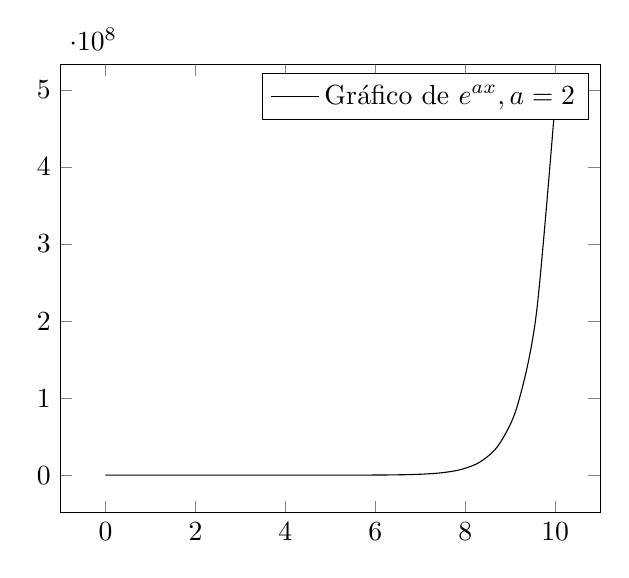
\begin{tikzpicture}
				\begin{axis}
					\addplot[ domain = 0:10, smooth,] {exp(2*x)}; \legend{ Gr\'afico de {$e^{ax}, a = 2$} }
				\end{axis}
			\end{tikzpicture}
			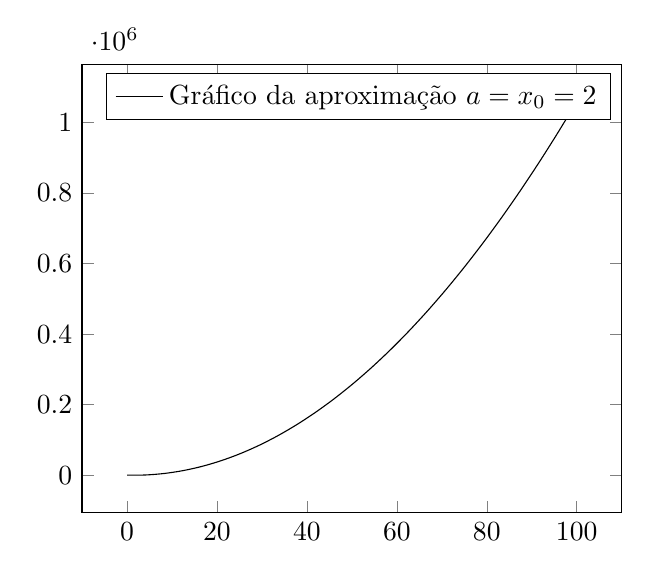
\begin{tikzpicture}
				\begin{axis}
					\addplot[ domain = 0:100, smooth, ]
					{exp(4) + 2*exp(4)*(x-2) + 4/2*exp(4)*(x-2)^2}; \legend{ Gr\'afico da aproxima\c c\~ao {$a=x_{0}=2$} }
				\end{axis}
			\end{tikzpicture}

		\item $\sin(ax)$
			\[
				\sin(ax) = \sin(ax_{0}) + a\cos(ax_{0})(x-x_{0}) - \frac{a^{2}\sin(ax_{0})}{2}(x-x_{0})^{2}.
			\]
			Vejamos, novamente, como o gr\'afico de ambas as fun\c c\~oes se comportam,
			tomando $x_{0}= \frac{\pi}{4}, a = 3$:
			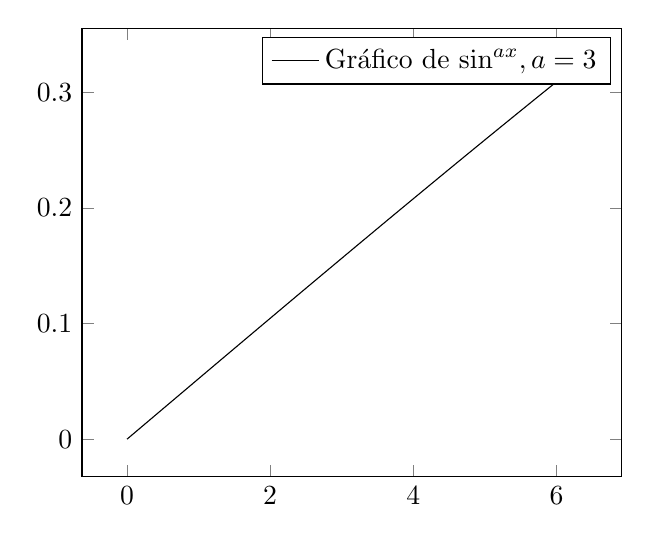
\begin{tikzpicture}
				\begin{axis}[]
					\addplot[ domain = 0:2*pi, smooth, ] {sin(3*x)}; \legend{ Gr\'afico de {$\sin^{ax}, a = 3$} }
				\end{axis}
			\end{tikzpicture}
			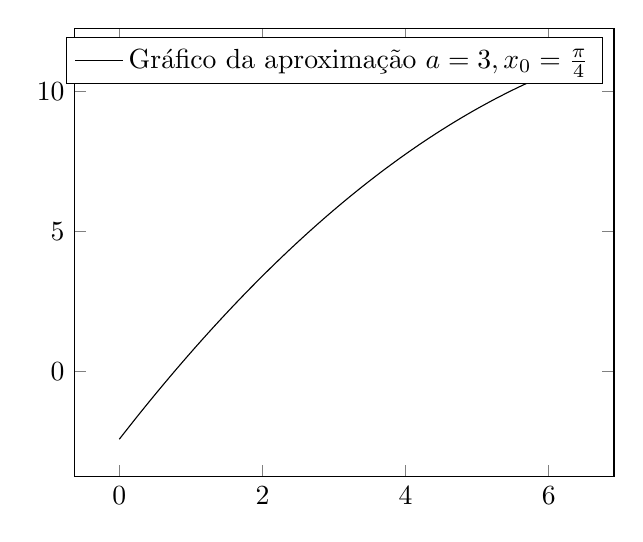
\begin{tikzpicture}
				\begin{axis}
					\addplot[ domain = 0:2*pi, smooth, ]
					{sin(3/4*pi) + 3*cos(3/4*pi)*(x-pi/4) - 9/2*sin(3/4*pi)*(x-pi/4)^2}; \legend{ Gr\'afico da aproxima\c c\~ao {$a=3, x_{0}=\frac{\pi}{4}$} }
				\end{axis}
			\end{tikzpicture}
	\end{itemize}
	\qedsymbol
\end{proof*}

\subsection{Taxas de Varia\c c\~ao.}
\subsubsection{Exerc\'icio 1.}
Com a aplica\c c\~ao da segunda lei de Newton, diga se o movimento da part\'icula
dada por
\[
	s(t) = (t^{2}+ e)ln(t), \quad t>0, \quad s(0) = 0
\]
\'e el\'astico.
\begin{proof*}
	Para determinar se um movimento el\'astico, \'e necess\'ario analisar sua segunda
	derivada. De forma expl\'icita, uma fun\c c\~ao de tempo x(t) descrevendo uma part\'icula
	ser\'a el\'astica se
	\[
		\ddot{x}(t) = -kx(t), \quad k\in\mathbb{R},
	\]
	em que $\ddot{x}(t)$ denota a segunda derivada de x com respeito a t, ou seja,
	sua acelera\c c\~ao com o tempo. Vamos aplicar esta ideia \`a fun\c c\~ao fornecida:
	\[
		a(t) = \frac{d^{2}}{dx^{2}}s(t) = 2\ln (t) -1 - \frac{e}{t^{2}}+ 4 \neq -kx(t)
	\]
	Portanto, o movimento n\~ao \'e el\'astico, pois n\~ao h\'a k que a fa\c ca
	satisfazer a equa\c c\~ao el\'astica. \qedsymbol
\end{proof*}

\subsection{M\'aximos e M\'inimos.}
\subsubsection{Exerc\'icio 1.}
Fa\c ca um estudo completo do comportamento das fun\c c\~oes abaixo, justificando
cada passagem e esbo\c cando o gr\'afico:
\begin{equation*}
	y = \frac{x}{x+1}, \quad g(x) = xe^{-3x}, \quad f(x) = 2x + 1 + e^{-x}
\end{equation*}
\begin{proof*}
	Come\c cando pela y, vamos observar as derivadas:
	\[
		\frac{dy}{dx}= \frac{x+1 - x}{(x+1)^{2}}= \frac{1}{(x+1)^{2}}> 0, \quad\forall x\in\mathbb{R},
	\]
	tal que a fun\c c\~ao \'e estritamente crescente e nunca atinge um m\'aximo. Al\'em
	disso, analisando sua segunda derivada, temos
	\[
		y^{''}= \frac{-2}{(x+1)^{3}}.
	\]
	Neste caso, \'e preciso ter um pouco mais de cuidado, pois, para $x > -1, (x+1)
	^{3} > 0$, tal que
	\[
		y^{''}< 0.
	\]
	No entanto, para $x < -1, (x + 1)^{3} < 0$ e
	\[
		y^{''}> 0.
	\]
	Em outras palavras, a fun\c c\~ao tem uma concavidade para cima quando x \'e
	menor que 1 e para baixo caso contr\'ario.

	Agora, com rela\c c\~ao \`a g(x), obtemos o seguinte:
	\[
		\frac{d g(x)}{dx}= -3xe^{-3x}+ e^{-3x}= e^{-3x}(-3x + 1).
	\]
	Como a exponencial \'e sempre positiva, o termo que determina se a derivada
	ser\'a positiva ou n\~ao \'e o -3x + 1. Com efeito, analisando ele, temos:
	\[
		-3x + 1 > 0 \Rightarrow x < \frac{1}{3}, \quad -3x + 1 < 0 \Rightarrow x > \frac{1}{3}.
	\]
	Disto, conclu\'imos que a fun\c c\~ao g \'e estritamente crescente para x
	menor que $\frac{1}{3}$ e estritamente decrescente para x maior que
	$\frac{1}{3}$. Ademais, no ponto $x = \frac{1}{3}$, ela tem um ponto de m\'aximo
	local, pois sua derivada \'e zero e ela come\c ca a diminuir \`a direita do ponto 
	(afinal, $x > \frac{1}{3}$ faz com que a fun\c c\~ao decres\c ca). 
	Por fim, analisando a segunda derivada,
	\[
		g^{''}(x) = -3e^{-3x}(-3x + 1) -3e^{-3x}= -3e^{-3x}(-3x + 1) = -3g^{'}(x).
	\]
	Com isto, podemos aplicar o estudo de sinal da primeira derivada para descobrir
	que ela ter\'a concavidade para baixo quando x for menor que $\frac{1}{3}$,
	pois $g^{'}(x) > 0$, mas multiplicar por -3 a torna negativa, e ser\'a concavidade
	para cima quando x for maior que $\frac{1}{3}$, visto que $g^{'}(x) < 0$, mas $-
	3g^{'}(x) > 0$ neste caso.

	Finalmente, analisemos a f:
	\[
		f^{'}(x) = 2 - e^{-x}.
	\]
	Neste caso, $f^{'}(x) > 0$ se $2 > e^{-x}$, ou seja, se $-\ln(2) < x$. Analogamente,
	$f^{'}(x) < 0$ se $-ln(2) > x$. Isto significa que quando $-\ln(2) < x$, a fun\c
	c\~ao ser\'a estritamente crescente, mas ser\'a estritamente decrescente
	quando $-\ln(2) > x.$ No ponto $-\ln(2) = x,$ a fun\c c\~ao possui um ponto de
	inflex\~ao que ser\'a um m\'inimo local, visto que a exponencial come\c car\'a
	a crescer e dominar a fun\c c\~ao, pois em $x > -\ln(2)$, ou seja, \`a direito do ponto de
	anulamento, a fun\c c\~ao \'e crescente. Com rela\c c\~ao \`a segunda derivada,
	temos:
	\[
		f^{''}(x) = e^{-x},
	\]
	uma fun\c c\~ao que \'e positiva para todo n\'umero x. Em outras palavras, ela
	tem uma concavidade para cima para todo x.

	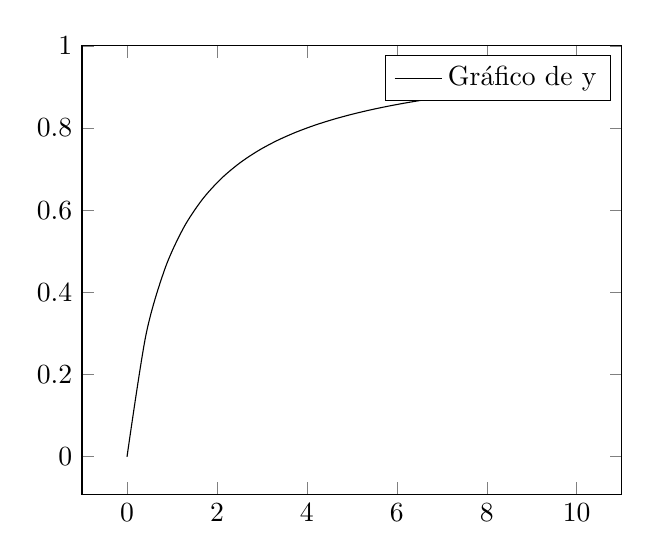
\begin{tikzpicture}
		\begin{axis}[]
			\addplot[ domain = 0:10, smooth, ] {x/(x+1)}; \legend{ Gr\'afico de y}
		\end{axis}
	\end{tikzpicture}
	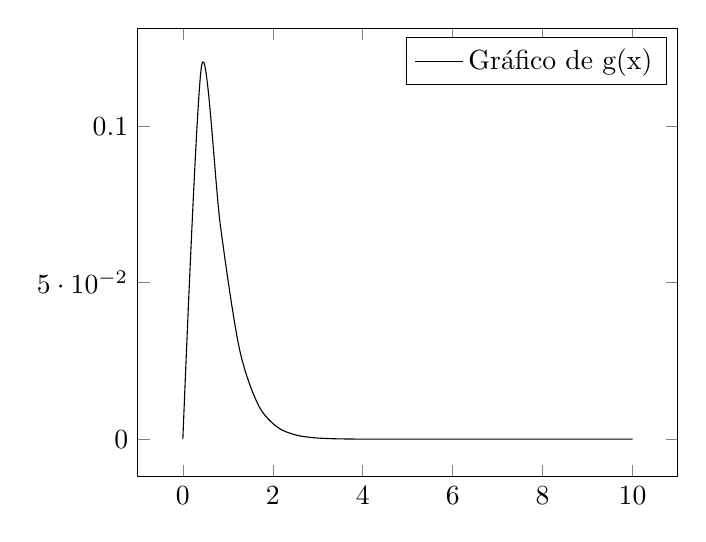
\begin{tikzpicture}
		\begin{axis}[]
			\addplot[ domain = 0:10, smooth, ] {x*exp(-3*x)}; \legend{ Gr\'afico de g(x)}
		\end{axis}
	\end{tikzpicture}

	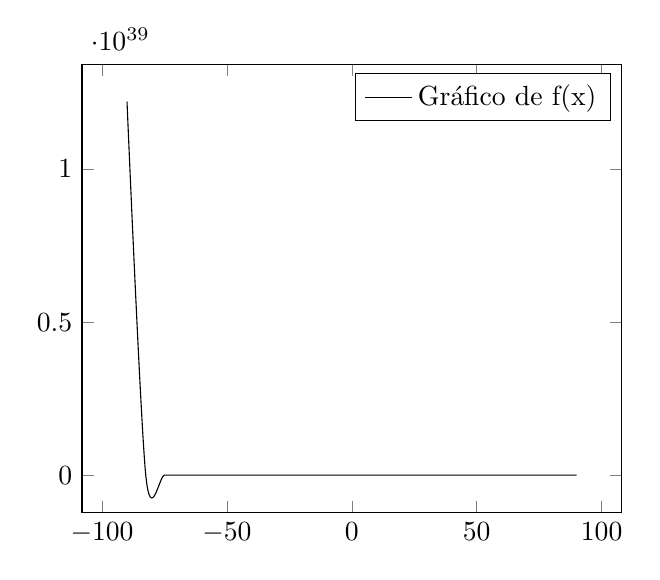
\begin{tikzpicture}
		\begin{axis}[]
			\addplot[ domain = -90:90, smooth, ] {2*x + 1 + exp(-x)}; \legend{ Gr\'afico de f(x) }
		\end{axis}
	\end{tikzpicture}
\end{proof*}
